\documentclass{article}

\usepackage{graphicx}
\usepackage{amsmath}
\usepackage{amssymb}
\usepackage{bm}
\usepackage{tikz}
\usetikzlibrary{arrows.meta,positioning,fit,calc}
\usepackage{algorithm}
\usepackage{algpseudocode}

\title{Geometric Regularization JEPA}
% \author{Siddharth Nayak}
% \date{July 2026}

\begin{document}

\maketitle

\section{Introduction and Motivation}

LeWorldModel (LeWM) is the first method to learn a stable JEPA
end-to-end from raw pixels without relying on stabilization heuristics.
The method uses a simple two-term objective that remains robust across
architectures and hyperparameter choices, while enabling efficient
logarithmic-time hyperparameter search.

The operation of LeWM can be separated into two stages. During training,
the model learns the latent consequences of real actions observed in
environment trajectories. During inference, the trained model is used
inside the Cross-Entropy Method (CEM) to search over previously unseen
continuous action sequences.


Assume that the training dataset contains environment transitions of the
form

\[
\left(
o_t,
\mathbf{a}_t,
o_{t+1}
\right),
\]

where \(o_t\) and \(o_{t+1}\) are consecutive observations and

\[
\mathbf{a}_t \in \mathbb{R}^{d_a}
\]

is the real continuous action executed between them.

The encoder maps the current observation to a latent representation:

\[
\mathbf{z}_t
=
\operatorname{enc}_{\theta}(o_t).
\]

The next observation is encoded as the target latent representation:

\[
\mathbf{z}_{t+1}
=
\operatorname{enc}_{\theta}(o_{t+1}).
\]

Conditioned on the current latent state and the real action from the
trajectory, the predictor estimates the next latent state:

\[
\hat{\mathbf{z}}_{t+1}
=
\operatorname{pred}_{\phi}
\left(
\mathbf{z}_t,
\mathbf{a}_t
\right).
\]

Therefore, during training, the predictor learns the mapping

\[
\left(
\mathbf{z}_t,
\mathbf{a}_t
\right)
\longmapsto
\mathbf{z}_{t+1}.
\]

The latent prediction loss compares the predicted next latent state with
the latent representation of the real next observation:

\[
\mathcal{L}_{\mathrm{pred}}
=
\left\|
\hat{\mathbf{z}}_{t+1}
-
\mathbf{z}_{t+1}
\right\|_2^2.
\]

Equivalently,

\[
\mathcal{L}_{\mathrm{pred}}
=
\left\|
\operatorname{pred}_{\phi}
\left(
\operatorname{enc}_{\theta}(o_t),
\mathbf{a}_t
\right)
-
\operatorname{enc}_{\theta}(o_{t+1})
\right\|_2^2.
\]

Importantly, CEM is not used during this training stage. The actions used
to train the predictor are the real actions recorded in the training
trajectories.


\paragraph{Problem}
The predictor conditions on raw actions through AdaLN - no explicit representation of what an action does or how valuable it is in the current state.



\section{Architecture and Loss Derivation}

We introduce an explicit action representation that captures not only the
raw action parameters, but also the effect of the action in the current
latent state.

\subsection{Action Encoder}

The continuous action is first mapped into an action embedding:

\[
\mathbf{u}_t
=
A_{\psi}(\mathbf{a}_t),
\]

where

\[
\mathbf{a}_t \in \mathbb{R}^{d_a},
\qquad
\mathbf{u}_t \in \mathbb{R}^{d_e},
\]

and \(A_{\psi}\) is a learnable action encoder.

The action embedding \(\mathbf{u}_t\) represents the raw continuous
action independently of the current state. However, the same action may
have different consequences in different states. We therefore introduce
a state-conditioned effect encoder.

\subsection{State-Conditioned Action-Effect Encoder}

The effect representation is defined as

\[
\mathbf{e}_t
=
H_{\eta}
\left(
\operatorname{sg}(\mathbf{z}_t),
\mathbf{u}_t
\right),
\]

where \(\operatorname{sg}(\cdot)\) denotes the stop-gradient operator.

Substituting the action encoder gives

\[
\mathbf{e}_t
=
H_{\eta}
\left(
\operatorname{sg}(\mathbf{z}_t),
A_{\psi}(\mathbf{a}_t)
\right).
\]

The stop-gradient operation prevents the action-effect objective from
changing the state representation through this branch. Consequently,
the effect encoder and action encoder must adapt to the geometry of the
learned state space rather than modifying the state encoder to simplify
the action representation.

The effect representation can therefore be interpreted as

\[
\mathbf{e}_t
\approx
\text{effect of executing }
\mathbf{a}_t
\text{ in state }
\mathbf{z}_t.
\]

We note that this terminology is the converse of the standard usage in
the Dreamer and APV lineage, where an \emph{action-conditional} world
model is one whose \emph{state} is conditioned on the raw action. Here it
is the action representation that is conditioned on the state.

\subsection{Effect-Conditioned Latent Predictor}

Instead of conditioning the predictor directly on the raw action, the
predictor receives the state-conditioned effect representation:

\[
\hat{\mathbf{z}}_{t+1}
=
P_{\phi}
\left(
\mathbf{z}_t,
\mathbf{e}_t
\right).
\]

Equivalently, the complete prediction pathway is

\[
\hat{\mathbf{z}}_{t+1}
=
P_{\phi}
\left(
\mathbf{z}_t,
H_{\eta}
\left(
\operatorname{sg}(\mathbf{z}_t),
A_{\psi}(\mathbf{a}_t)
\right)
\right).
\]

This replaces direct raw-action conditioning,

\[
\hat{\mathbf{z}}_{t+1}
=
P_{\phi}(\mathbf{z}_t,\mathbf{a}_t),
\]

with explicit effect-based conditioning,

\[
\mathbf{a}_t
\longrightarrow
\mathbf{u}_t
\longrightarrow
\mathbf{e}_t
\longrightarrow
\hat{\mathbf{z}}_{t+1}.
\]

\subsection{Latent Prediction Loss}

The predicted next latent state is trained to match the encoded next
observation:

\[
\mathbf{z}_{t+1}
=
\operatorname{enc}_{\theta}(o_{t+1}).
\]

The prediction loss is

\[
\mathcal{L}_{\mathrm{pred}}
=
\left\|
\hat{\mathbf{z}}_{t+1}
-
\operatorname{sg}(\mathbf{z}_{t+1})
\right\|_2^2.
\]

Substituting the complete architecture gives

\[
\mathcal{L}_{\mathrm{pred}}
=
\left\|
P_{\phi}
\left(
\mathbf{z}_t,
H_{\eta}
\left(
\operatorname{sg}(\mathbf{z}_t),
A_{\psi}(\mathbf{a}_t)
\right)
\right)
-
\operatorname{sg}(\mathbf{z}_{t+1})
\right\|_2^2.
\]

This objective trains the action encoder, effect encoder, and predictor
to represent the transition induced by the observed action.

\subsection{State-Action Value Head}

To organize the action-effect space according to control relevance, we
introduce a state-action value function:

\[
\hat{Q}_t
=
Q_{\omega}
\left(
\operatorname{sg}(\mathbf{z}_t),
\mathbf{e}_t
\right).
\]

Equivalently,

\[
\hat{Q}_t
=
Q_{\omega}
\left(
\operatorname{sg}(\mathbf{z}_t),
H_{\eta}
\left(
\operatorname{sg}(\mathbf{z}_t),
A_{\psi}(\mathbf{a}_t)
\right)
\right).
\]

The value head estimates how useful the effect of action
\(\mathbf{a}_t\) is when executed in state \(\mathbf{z}_t\).

A one-step temporal-difference target can be defined as

\[
y_t
=
r_t
+
\gamma
\max_{\mathbf{a}'}
Q_{\bar{\omega}}
\left(
\operatorname{sg}(\mathbf{z}_{t+1}),
\mathbf{e}_{t+1}'
\right),
\]

where

\[
\mathbf{e}_{t+1}'
=
H_{\bar{\eta}}
\left(
\operatorname{sg}(\mathbf{z}_{t+1}),
A_{\bar{\psi}}(\mathbf{a}')
\right),
\]

and the barred parameters denote slowly updated target networks.

The Q-value regression loss is

\[
\mathcal{L}_{Q}
=
\left(
Q_{\omega}
\left(
\operatorname{sg}(\mathbf{z}_t),
\mathbf{e}_t
\right)
-
\operatorname{sg}(y_t)
\right)^2.
\]

For continuous actions, the maximization over \(\mathbf{a}'\) is generally
not computed exactly. It may instead be approximated using CEM:

\[
\mathbf{a}_{t+1}^{*}
\approx
\operatorname{CEM}
\left[
Q_{\bar{\omega}}
\left(
\operatorname{sg}(\mathbf{z}_{t+1}),
H_{\bar{\eta}}
\left(
\operatorname{sg}(\mathbf{z}_{t+1}),
A_{\bar{\psi}}(\mathbf{a}')
\right)
\right)
\right].
\]

The target then becomes

\[
y_t
=
r_t
+
\gamma
Q_{\bar{\omega}}
\left(
\operatorname{sg}(\mathbf{z}_{t+1}),
\mathbf{e}_{t+1}^{*}
\right).
\]

\subsection{Value-Shaped Effect Representation}

The Q-value loss is allowed to update the action encoder and effect
encoder:

\[
\nabla_{\psi,\eta}\mathcal{L}_{Q}
\neq
0.
\]

Therefore, the effect representation is shaped not only to predict the
next latent state, but also to preserve distinctions that are useful for
control.

The gradient pathway is

\[
\mathcal{L}_{Q}
\longrightarrow
Q_{\omega}
\longrightarrow
\mathbf{e}_t
\longrightarrow
H_{\eta}
\longrightarrow
A_{\psi}.
\]

At the same time, because the state input is stop-gradient,

\[
\nabla_{\theta}^{(Q)} \mathcal{L}_{Q}
=
0,
\]

so the Q-objective does not directly reshape the visual state encoder.

\subsection{Geometric Regularization}

Training the action-effect representation only through a value objective
may produce a degenerate geometry. In particular, several distinct
high-value actions available at the same state may be mapped to nearly
the same effect representation because the value head does not need to
distinguish between them.

Formally, consider the state-conditioned action-effect encoder

\[
\mathbf{e}_t
=
H_{\eta}
\left(
\operatorname{sg}(\mathbf{z}_t),
A_{\psi}(\mathbf{a}_t)
\right).
\]

For a fixed state \(\mathbf{z}_t\), define the complete action-to-effect
mapping as

\[
F_t(\mathbf{a})
=
H_{\eta}
\left(
\operatorname{sg}(\mathbf{z}_t),
A_{\psi}(\mathbf{a})
\right).
\]

Consider a small perturbation
\(\Delta \mathbf{a}\) around the action \(\mathbf{a}_t\). A first-order
Taylor expansion gives

\[
F_t(\mathbf{a}_t + \Delta \mathbf{a})
\approx
F_t(\mathbf{a}_t)
+
\mathbf{J}_t \Delta \mathbf{a},
\]

where

\[
\mathbf{J}_t
=
\left.
\frac{\partial F_t(\mathbf{a})}
{\partial \mathbf{a}}
\right|_{\mathbf{a}=\mathbf{a}_t}
\in
\mathbb{R}^{d_e \times d_a}
\]

is the Jacobian of the effect representation with respect to the
continuous action.

The corresponding local change in effect space is therefore

\[
\Delta \mathbf{e}
\approx
\mathbf{J}_t \Delta \mathbf{a}.
\]

Its squared Euclidean norm is

\[
\left\|
\Delta \mathbf{e}
\right\|_2^2
=
\left\|
\mathbf{J}_t \Delta \mathbf{a}
\right\|_2^2.
\]

Expanding this expression gives

\[
\left\|
\Delta \mathbf{e}
\right\|_2^2
=
\Delta \mathbf{a}^{\top}
\mathbf{J}_t^{\top}
\mathbf{J}_t
\Delta \mathbf{a}.
\]

The matrix

\[
\mathbf{G}_t
=
\mathbf{J}_t^{\top}\mathbf{J}_t
\in
\mathbb{R}^{d_a \times d_a}
\]

is the local Gram matrix induced by the action-effect mapping. It defines
the local metric placed on the continuous action space by the learned
effect representation.

The diagonal entries satisfy

\[
[\mathbf{G}_t]_{ii}
=
\left\|
\frac{\partial \mathbf{e}_t}
{\partial a_{t,i}}
\right\|_2^2,
\]

and therefore measure the local sensitivity of the effect representation
to the \(i\)-th action dimension.

The off-diagonal entries satisfy

\[
[\mathbf{G}_t]_{ij}
=
\left(
\frac{\partial \mathbf{e}_t}
{\partial a_{t,i}}
\right)^{\top}
\left(
\frac{\partial \mathbf{e}_t}
{\partial a_{t,j}}
\right),
\qquad
i \neq j,
\]

and measure the local coupling between action dimensions \(i\) and \(j\)
inside the effect space.

To preserve distinct continuous action directions, we encourage the
Jacobian columns to be mutually orthogonal and equal in norm. This
corresponds to the condition

\[
\mathbf{J}_t^{\top}\mathbf{J}_t
\approx
\alpha \mathbf{I}_{d_a},
\qquad
\alpha > 0.
\]

Under this condition,

\[
\left\|
\Delta \mathbf{e}
\right\|_2^2
\approx
\alpha
\left\|
\Delta \mathbf{a}
\right\|_2^2.
\]

Thus, small distances and independent directions in the original action
space are approximately preserved in the learned effect space, up to a
global scaling factor \(\alpha\).

The geometric regularization loss is therefore defined as

\[
\mathcal{L}_{\mathrm{geo}}
=
\left\|
\mathbf{J}_t^{\top}\mathbf{J}_t
-
\alpha \mathbf{I}_{d_a}
\right\|_F^2.
\]

For a minibatch of \(B\) transitions, the loss becomes

\[
\mathcal{L}_{\mathrm{geo}}
=
\frac{1}{B}
\sum_{t=1}^{B}
\left\|
\mathbf{J}_t^{\top}\mathbf{J}_t
-
\alpha \mathbf{I}_{d_a}
\right\|_F^2.
\]

The geometric loss complements the value objective. The value loss
organizes effect representations according to control utility, while the
Jacobian regularizer prevents distinct local action directions from
collapsing into the same representation.

Beyond preventing collapse, the isometry condition has a planning-specific
justification. CEM proposes candidate action sequences from an isotropic
distribution in raw action space, while the candidates are scored in effect
space through \(Q_{\omega}\). If \(\mathbf{J}_t\) is ill-conditioned, the
isotropic proposal distribution is mapped to a highly eccentric ellipsoid,
the elite set is selected almost entirely by the high-gain directions, and
the refitted proposal distribution receives no informative update along the
low-gain directions. Enforcing \(\mathbf{G}_t \approx \alpha \mathbf{I}\)
keeps the search geometry of the planner aligned with the geometry of the
representation it searches over.

The complete objective can therefore be written as

\[
\mathcal{L}_{\mathrm{total}}
=
\mathcal{L}_{\mathrm{LeWM}}
+
\lambda_Q \mathcal{L}_Q
+
\lambda_{\mathrm{geo}}
\mathcal{L}_{\mathrm{geo}}.
\]

\section{Related Papers}

We group prior work into three families: latent world models that condition
on raw actions, methods that learn an explicit action representation, and
Jacobian-based geometric regularizers. Our components individually have
precedent in each family. The contribution is located in the routing of the
value gradient and in the object on which the geometric constraint acts.

\subsection{Latent World Models with Raw Action Conditioning}

\paragraph{TD-MPC2}
TD-MPC2 learns a decoder-free latent world model by combining a joint-embedding prediction loss with reward and TD-value regression on a shared trunk, and derives a policy by sampling-based trajectory optimization (MPPI) in latent space with the learned terminal value bootstrapping beyond the planning horizon. Actions enter its dynamics, reward, and value heads by raw concatenation, so the only learned embeddings in the model are the latent state and, in the multitask setting, a task identifier. We differ in two respects:
\begin{itemize}
  \item \textbf{Where value supervision enters.} In TD-MPC2 the reward and value objectives share a trunk with the encoder, so value gradients reshape the state representation itself, and actions are never given a representation of their own. We invert both choices: we introduce an explicit state-conditioned action-effect representation $e_t = H_\eta(\mathrm{sg}(z_t), A_\psi(a_t))$ and route the value gradient into it, while stop-gradients keep the state encoder value-agnostic and trained by latent prediction alone.
  \item \textbf{What the geometry constraint acts on.} TD-MPC2 constrains only the state latent, via a simplicial projection (SimNorm) that bounds its norm and biases it toward sparsity. We instead constrain the geometry of the action-effect space, penalizing $\|J_t^\top J_t - \alpha I\|_F^2$ so that the local action-to-effect map remains well conditioned and the planner's isotropic proposal distribution is not distorted in effect space.
\end{itemize}
We also adopt two of its practical lessons. Its policy prior exists to make the
TD target affordable by replacing the intractable $\max_{a'}$ with a single
forward pass, which is directly relevant to our CEM-based target, and its
discrete regression of value in a log-transformed space removes the dependence
of the value loss magnitude on reward scale.

\paragraph{APV}
APV pre-trains an action-free latent video prediction model on videos from
unrelated domains and then fine-tunes it into an action-conditional world model
for control. Its action-conditional stage conditions the \emph{state} on the raw
action, both in the recurrent cell $h^{AC}_t = f_\theta(h^{AC}_{t-1}, z^{AC}_{t-1}, a_{t-1})$
and in the posterior, with no function applied to $a_{t-1}$ at any point. It is
therefore an instance of the raw-conditioning pattern rather than an action
representation method, and we cite it as such.

APV is nonetheless directly relevant to our stop-gradient design. The authors
report that the naive fine-tuning scheme, which initializes the action-conditional
model from the pre-trained action-free weights and trains everything jointly,
rapidly erases the knowledge held in the pre-trained representation. Their remedy
is architectural separation: a new action-conditional model is stacked on top and
the action-free branch is decoupled from the downstream objective. This is
empirical precedent for the claim underlying $\nabla_{\theta}^{(Q)}\mathcal{L}_Q = 0$,
namely that a representation trained by prediction degrades when a task-shaped
objective is permitted to reshape it. Our mechanism differs, a gradient block
rather than an architectural stack, but the underlying claim is the same.

\subsection{Learned Action Representations}

\paragraph{Action embedding learning}
Learned action representations inside dynamics models are well established.
Chandak et al. and Dynamics-Aware Embeddings (DynE) learn continuous action
embeddings shaped by forward or inverse dynamics, and SALE learns a
state-conditioned state-action embedding $z_{sa}$ that is consumed by the value
function. We regard the existence of a learned, state-conditioned action encoder
as established apparatus rather than as a contribution. What distinguishes our
formulation is the supervision reaching it: in all of the above the embedding is
shaped by dynamics or by an inverse-dynamics objective, and the value signal is
either absent or explicitly blocked from the embedding. We allow the value
gradient to reach $A_\psi$ and $H_\eta$, and we additionally constrain the
geometry of the resulting space.

\paragraph{PreLAR}
PreLAR also equips a world model with a learnable action representation, encoding
adjacent observation pairs into an implicit action code so that a Dreamer-style
model can be pre-trained as action-conditional from action-free video, with an
action-state consistency loss aligning the code with real actions at fine-tuning
time. It is the direct successor to APV and closes the gap that APV leaves open,
namely that pre-training without actions transfers poorly into an
action-conditional model. We share the premise that a world model benefits from an
explicit action representation rather than raw action conditioning, but differ in
what shapes it and why:
\begin{itemize}
  \item \textbf{Supervision.} PreLAR's representation is shaped entirely by
  dynamics prediction and self-supervised consistency. No value or return signal
  reaches it. Ours is shaped by $\mathcal{L}_Q$.
  \item \textbf{Purpose.} PreLAR's goal is transfer, recovering action-conditional
  structure from unlabelled video to improve sample efficiency. Ours is planning
  quality under a fixed sample budget.
  \item \textbf{Consumer.} PreLAR's actor-critic operates in imagination on a
  reconstruction-based RSSM. There is no sampling-based planner, so the
  conditioning of the action-to-effect map has no bearing on its behaviour and no
  analogue of $\mathcal{L}_{\mathrm{geo}}$ is required.
\end{itemize}

\subsection{Jacobian-Based Geometric Regularization}

\paragraph{OroJaR}
OroJaR regularizes the Jacobian of a generator with respect to its latent input,
penalizing the pairwise inner products of Jacobian columns so that each latent
dimension controls an independent factor of variation. Written as a Gram matrix
penalty, OroJaR minimizes $\|J^\top J - \mathrm{diag}(J^\top J)\|_F^2$, and the paper
is explicit that no constraint is placed on the individual column norms. Our
$\mathcal{L}_{\text{geo}} = \|J_t^\top J_t - \alpha I\|_F^2$ is the same device applied
to a different object under a strictly stronger condition. We differ in three respects:
\begin{itemize}
  \item \textbf{Isometry rather than orthogonality.} OroJaR leaves the diagonal of
  $J^\top J$ free, which is a conformal condition: a map with
  $J^\top J = \mathrm{diag}(100, 10^{-2})$ is OroJaR-optimal yet arbitrarily
  ill-conditioned. Pinning the diagonal instead equalizes the singular values of
  $J_t$ and bounds its condition number.
  \item \textbf{Motivated by planning, not interpretability.} CEM proposes candidate
  actions from an isotropic distribution in raw action space, so an ill-conditioned
  action-to-effect map turns that proposal ball into an eccentric ellipsoid and the
  planner spends nearly its entire sample budget on a single effect direction.
  Uniform gain across directions is therefore essential here and irrelevant to
  disentanglement, where factors are expected to carry their natural scales.

\end{itemize}


\subsection{Summary of Positioning}

Each ingredient of the proposed method has precedent. Learned and
state-conditioned action embeddings appear in DynE, SALE, and PreLAR. Value
shaping of a latent world model appears in VAML, MuZero, and TD-MPC2. Jacobian
orthogonality penalties appear in OroJaR. What is not addressed in prior work is
the conjunction and the causal question it permits: whether routing the value
gradient specifically into a state-conditioned action-effect encoder, with the
geometry of that encoder constrained for planner conditioning, improves planning
return under a fixed sample budget relative to routing the same signal elsewhere.
The parameter-matched routing variants isolate exactly this question.

\begin{figure}
    \centering
    \includegraphics[width=1.2\linewidth]{figures/geometric_regularization_jepa_architecture.png}
    \caption{Proposed architecture}
    \label{fig:architecture}
\end{figure}

\subsection{Choice of $\alpha$}
    Let's consider State-Dependent Target via a Decoupled Estimator. The geometric regularizer introduced in the previous section requires a scale $\alpha$ against which the local Gram matrix $\mathbf{G}_t = \mathbf{J}_t^\top \mathbf{J}_t$ is compared. We first show that allowing $\alpha$ to adapt freely to $\mathbf{G}_t$ collapses the regularizer to a strictly weaker objective that no longer penalizes representational collapse, which motivates a decoupled, per-state formulation.

    \paragraph{Degeneracy of a freely-fit $\alpha$.}
        For a fixed $\mathbf{G}_t \in \mathbb{R}^{d_a \times d_a}$, consider the value
        of $\alpha$ that minimizes $\|\mathbf{G}_t - \alpha \mathbf{I}_{d_a}\|_F^2$.
        Expanding the norm,
        \[
        \|\mathbf{G}_t - \alpha \mathbf{I}_{d_a}\|_F^2
        = \|\mathbf{G}_t\|_F^2 - 2\alpha\,\mathrm{tr}(\mathbf{G}_t) + \alpha^2 d_a.
        \]
        Differentiating with respect to $\alpha$ and setting the result to zero gives
        \[
        \alpha^\star_t = \frac{\mathrm{tr}(\mathbf{G}_t)}{d_a}.
        \]
        Substituting $\alpha^\star_t$ back into the loss,
        \[
        \min_{\alpha} \|\mathbf{G}_t - \alpha \mathbf{I}_{d_a}\|_F^2
        = \|\mathbf{G}_t\|_F^2 - \frac{\mathrm{tr}(\mathbf{G}_t)^2}{d_a}
        = d_a \cdot \mathrm{Var}(\lambda_1, \dots, \lambda_{d_a}),
        \]
        where $\lambda_1, \dots, \lambda_{d_a}$ are the eigenvalues of $\mathbf{G}_t$
        (symmetric positive semi-definite, since $\mathbf{G}_t = \mathbf{J}_t^\top
        \mathbf{J}_t$). This quantity depends only on the \emph{dispersion} of the
        eigenvalues, not their magnitude, and vanishes whenever
        $\lambda_1 = \dots = \lambda_{d_a}$ -- including the degenerate case
        $\mathbf{G}_t = \mathbf{0}$, i.e.\ $\mathbf{J}_t = \mathbf{0}$.

    \begin{quote}
        \itshape
        Consequently, any $\alpha_t$ that instantaneously tracks $\mathbf{G}_t$; a
        per-sample closed form $\alpha_t = \mathrm{tr}(\mathbf{G}_t)/d_a$, a network
        trained jointly on $\mathcal{L}_{geo}$ itself, or a single global scalar
        optimized by gradient descent on the same batch; reduces $\mathcal{L}_{geo}$
        to an anisotropy-only penalty that imposes \emph{no} pressure against
        collapsing the action-effect Jacobian to zero. This holds even under a
        stop-gradient on the $\alpha_t$ computation: by the envelope theorem,
        $\partial/\partial \mathbf{G}_t \left[\min_\alpha \|\mathbf{G}_t -
        \alpha\mathbf{I}\|_F^2\right]$ equals the gradient with $\alpha$ held fixed at
        $\alpha^\star_t$, since $\partial \|\mathbf{G}_t - \alpha\mathbf{I}\|_F^2 /
        \partial \alpha = 0$ at $\alpha = \alpha_t^\star$.
    \end{quote}


    \paragraph{Proposed formulation.}
        We let $\alpha$ vary across states for adaptivity, but decouple its
        estimation from the parameters being regularized, following the
        target-network pattern already used for $\bar{Q}_{\bar\omega}$,
        $\bar{H}_{\bar\eta}$, and $\bar{A}_{\bar\psi}$.
         
        Define a scalar head with a positivity floor,
        \[
        \alpha_\xi(\mathbf{z}) = \mathrm{softplus}\big(\mathrm{MLP}_\xi(\mathbf{z})\big)
        + \alpha_{\min}, \qquad \alpha_{\min} > 0,
        \]
        maintained as a fast copy $\xi$ and a slowly-updated target copy $\bar\xi$,
        \[
        \bar\xi \leftarrow (1-\tau)\,\bar\xi + \tau\,\xi, \qquad \tau \ll 1.
        \]
         
        The fast head is trained on an auxiliary regression loss toward the current
        per-sample trace target, and is never updated through $\mathcal{L}_{geo}$
        directly:
        \[
        \mathcal{L}_\alpha = \frac{1}{B}\sum_{t=1}^{B}
        \Big(\alpha_\xi(\mathrm{sg}(\mathbf{z}_t))
        - \mathrm{sg}\big(\mathrm{tr}(\mathbf{J}_t^\top \mathbf{J}_t)/d_a\big)\Big)^2.
        \]
         
        The geometric loss is then evaluated against the \emph{target} network only,
        \[
        \alpha_t = \alpha_{\bar\xi}(\mathrm{sg}(\mathbf{z}_t)), \qquad
        \mathcal{L}_{geo} = \frac{1}{B}\sum_{t=1}^{B}
        \big\|\mathbf{J}_t^\top \mathbf{J}_t - \alpha_t \mathbf{I}_{d_a}\big\|_F^2,
        \]
        with no gradient flowing into $\bar\xi$ except through the Polyak update. The
        complete objective becomes
        \[
        \mathcal{L}_{total} = \mathcal{L}_{LeWM} + \lambda_Q \mathcal{L}_Q
        + \lambda_{geo} \mathcal{L}_{geo} + \lambda_\alpha \mathcal{L}_\alpha.
        \]
   
\subsection{Hutchinson Estimation of the Jacobian Regularizer}

The geometric objective introduced above is
\[
\mathcal{L}_{\mathrm{geo},t}
=
\left\|
\mathbf{J}_t^{\top}\mathbf{J}_t
-
\alpha_t\mathbf{I}_{d_a}
\right\|_F^2,
\]
where \(\alpha_t=\alpha_{\bar\xi}(\operatorname{sg}(\mathbf{z}_t))\) is
provided by the slowly updated scale network defined in the previous
subsection. This subsection changes only how the loss is evaluated; it does
not change the definition or training procedure of \(\alpha_t\).

Explicitly constructing
\[
\mathbf{J}_t
=
\frac{\partial F_t(\mathbf{a}_t)}{\partial \mathbf{a}_t}
\in\mathbb{R}^{d_e\times d_a}
\]
and then forming
\[
\mathbf{G}_t
=
\mathbf{J}_t^{\top}\mathbf{J}_t
\in\mathbb{R}^{d_a\times d_a}
\]
can be expensive for high-dimensional action spaces. We therefore use
Hutchinson's identity to estimate the same Frobenius-norm objective using
only products with the Jacobian.

\paragraph{Trace representation of the loss.}
Define the symmetric residual matrix
\[
\mathbf{M}_t
=
\mathbf{G}_t-
\alpha_t\mathbf{I}_{d_a}
=
\mathbf{J}_t^{\top}\mathbf{J}_t
-
\alpha_t\mathbf{I}_{d_a}.
\]
The exact geometric loss can be written as
\[
\begin{aligned}
\mathcal{L}_{\mathrm{geo},t}
&=
\|\mathbf{M}_t\|_F^2 \\
&=
\operatorname{tr}(\mathbf{M}_t^{\top}\mathbf{M}_t) \\
&=
\operatorname{tr}(\mathbf{M}_t^2),
\end{aligned}
\]
where the last equality follows because \(\mathbf{M}_t\) is symmetric.

Let
\[
\bm{\epsilon}_{t,k}\in\mathbb{R}^{d_a}
\]
be an independent random probe satisfying
\[
\mathbb{E}
\left[
\bm{\epsilon}_{t,k}\bm{\epsilon}_{t,k}^{\top}
\right]
=
\mathbf{I}_{d_a}.
\]
We use Rademacher probes, whose coordinates are sampled independently as
\[
\epsilon_{t,k,i}
=
\begin{cases}
+1, & \text{with probability } \tfrac{1}{2},\\
-1, & \text{with probability } \tfrac{1}{2}.
\end{cases}
\]
For any symmetric matrix \(\mathbf{A}\), Hutchinson's identity gives
\[
\mathbb{E}_{\bm{\epsilon}}
\left[
\bm{\epsilon}^{\top}\mathbf{A}\bm{\epsilon}
\right]
=
\operatorname{tr}(\mathbf{A}).
\]
Applying it with \(\mathbf{A}=\mathbf{M}_t^2\) yields
\[
\begin{aligned}
\mathcal{L}_{\mathrm{geo},t}
&=
\mathbb{E}_{\bm{\epsilon}}
\left[
\bm{\epsilon}^{\top}\mathbf{M}_t^2\bm{\epsilon}
\right] \\
&=
\mathbb{E}_{\bm{\epsilon}}
\left[
\|\mathbf{M}_t\bm{\epsilon}\|_2^2
\right].
\end{aligned}
\]
Substituting the definition of \(\mathbf{M}_t\),
\[
\boxed{
\mathcal{L}_{\mathrm{geo},t}
=
\mathbb{E}_{\bm{\epsilon}}
\left[
\left\|
\mathbf{J}_t^{\top}
\left(
\mathbf{J}_t\bm{\epsilon}
\right)
-
\alpha_t\bm{\epsilon}
\right\|_2^2
\right]
}.
\]
Thus, the random probe tests whether the local metric acts on an arbitrary
action-space direction as
\[
\mathbf{J}_t^{\top}\mathbf{J}_t\bm{\epsilon}
\approx
\alpha_t\bm{\epsilon}.
\]
When this holds for all directions, the Jacobian columns are approximately
orthogonal and equal in norm, and the local action geometry is preserved up
to the scale \(\alpha_t\).

\paragraph{Matrix-free Monte Carlo estimator.}
For each probe, define
\[
\mathbf{v}_{t,k}
=
\mathbf{J}_t\bm{\epsilon}_{t,k}
\in\mathbb{R}^{d_e}
\]
and
\[
\mathbf{w}_{t,k}
=
\mathbf{J}_t^{\top}\mathbf{v}_{t,k}
=
\mathbf{J}_t^{\top}\mathbf{J}_t\bm{\epsilon}_{t,k}
\in\mathbb{R}^{d_a}.
\]
The first quantity is computed with a Jacobian--vector product, and the
second with a vector--Jacobian product. Neither \(\mathbf{J}_t\) nor
\(\mathbf{G}_t\) is explicitly formed.

Using \(K\) independent probes, the per-transition estimator is
\[
\widehat{\mathcal{L}}_{\mathrm{geo},t}
=
\frac{1}{K}
\sum_{k=1}^{K}
\left\|
\mathbf{w}_{t,k}
-
\alpha_t\bm{\epsilon}_{t,k}
\right\|_2^2.
\]
For a minibatch of \(B\) transitions,
\[
\boxed{
\widehat{\mathcal{L}}_{\mathrm{geo}}
=
\frac{1}{BK}
\sum_{t=1}^{B}
\sum_{k=1}^{K}
\left\|
\mathbf{J}_t^{\top}
\left(
\mathbf{J}_t\bm{\epsilon}_{t,k}
\right)
-
\alpha_t\bm{\epsilon}_{t,k}
\right\|_2^2
}.
\]
Because the probes are independent of the model parameters and satisfy
\(\mathbb{E}[\bm{\epsilon}\bm{\epsilon}^{\top}]=\mathbf{I}\),
\[
\mathbb{E}_{\bm{\epsilon}}
\left[
\widehat{\mathcal{L}}_{\mathrm{geo}}
\right]
=
\mathcal{L}_{\mathrm{geo}}.
\]
The estimator is therefore unbiased for the exact geometric loss. During
this computation, \(\alpha_t\) is treated as a target value: no gradient is
propagated into \(\bar\xi\) through
\(\widehat{\mathcal{L}}_{\mathrm{geo}}\).

\paragraph{Estimating the trace target for the scale network.}
The auxiliary objective in the previous subsection uses
\[
s_t
=
\frac{1}{d_a}
\operatorname{tr}
\left(
\mathbf{J}_t^{\top}\mathbf{J}_t
\right).
\]
The same probes give
\[
\begin{aligned}
\operatorname{tr}
\left(
\mathbf{J}_t^{\top}\mathbf{J}_t
\right)
&=
\mathbb{E}_{\bm{\epsilon}}
\left[
\bm{\epsilon}^{\top}
\mathbf{J}_t^{\top}\mathbf{J}_t
\bm{\epsilon}
\right] \\
&=
\mathbb{E}_{\bm{\epsilon}}
\left[
\|\mathbf{J}_t\bm{\epsilon}\|_2^2
\right].
\end{aligned}
\]
Hence,
\[
\boxed{
\widehat{s}_t
=
\frac{1}{Kd_a}
\sum_{k=1}^{K}
\|\mathbf{v}_{t,k}\|_2^2
=
\frac{1}{Kd_a}
\sum_{k=1}^{K}
\|\mathbf{J}_t\bm{\epsilon}_{t,k}\|_2^2
}
\]
is an unbiased estimate of the per-state mean squared singular value. The
auxiliary loss becomes
\[
\widehat{\mathcal{L}}_{\alpha}
=
\frac{1}{B}
\sum_{t=1}^{B}
\left(
\alpha_{\xi}
\left(
\operatorname{sg}(\mathbf{z}_t)
\right)
-
\operatorname{sg}(\widehat{s}_t)
\right)^2.
\]
The stop-gradient on \(\widehat{s}_t\) ensures that this auxiliary
regression updates only the fast scale head \(\xi\); it does not update the
action-effect encoder through the trace target.

\paragraph{Why no U-statistic is required here.}
The estimator above is applied directly to
\[
\|\mathbf{G}_t-\alpha_t\mathbf{I}\|_F^2
\]
through \(\|\mathbf{M}_t\bm{\epsilon}\|_2^2\). It never forms the square of
an estimated trace. Consequently, a single probe already gives an unbiased
estimate of the full geometric loss, and no pairwise U-statistic is needed.
A U-statistic would be required only after algebraically decomposing the
objective into separate terms containing
\(\operatorname{tr}(\mathbf{G}_t)^2\).

\paragraph{Computational considerations.}
Each probe requires one Jacobian--vector product and one vector--Jacobian
product. The estimator is most useful when \(K\ll d_a\). For the
low-dimensional action spaces common in many continuous-control benchmarks,
forming the exact Jacobian may be cheaper and produces a zero-variance loss.
For higher-dimensional action spaces, a small number of probes provides a
matrix-free approximation. In either case, because the loss itself depends on
\(\mathbf{J}_t\), updating the parameters of \(A_{\psi}\) and \(H_{\eta}\)
requires differentiating through these products, introducing one level of
second-order automatic differentiation.

The resulting stochastic training objective is
\[
\mathcal{L}_{\mathrm{total}}
=
\mathcal{L}_{\mathrm{LeWM}}
+
\lambda_Q\mathcal{L}_Q
+
\lambda_{\mathrm{geo}}
\widehat{\mathcal{L}}_{\mathrm{geo}}
+
\lambda_{\alpha}
\widehat{\mathcal{L}}_{\alpha}.
\]


\providecommand{\sg}{\operatorname{sg}}

\section{Addendum: Open Issue in the Treatment of $\alpha$}
\label{sec:addendum-alpha}

This addendum is written for discussion and is deliberate\-ly kept separate
from Sections~3.5 and 3.6, which are unchanged. It states an objection to the
scheme as currently formulated, records why the target-network construction
does not by itself answer that objection, and sets out two candidate
resolutions together with the trade-off between them. It closes with two
technical points (estimator variance and a feasibility condition) that are
independent of which resolution is adopted.

\subsection{Statement of the objection}
\label{sec:addendum-objection}

The degeneracy argument of Section~3.5 establishes that for a fixed
$\mathbf{G}_t$,
\[
  \min_{\alpha}\bigl\|\mathbf{G}_t-\alpha\mathbf{I}_{d_a}\bigr\|_F^2
  \;=\;
  \|\mathbf{G}_t\|_F^2-\frac{\operatorname{tr}(\mathbf{G}_t)^2}{d_a}
  \;=\;
  d_a\cdot\operatorname{Var}(\lambda_1,\dots,\lambda_{d_a}),
\]
a quantity that is invariant to the overall magnitude of the spectrum and
that vanishes at $\mathbf{G}_t=\mathbf{0}$. Any $\alpha_t$ that tracks
$\operatorname{tr}(\mathbf{G}_t)/d_a$ therefore reduces $\mathcal{L}_{geo}$ to
a penalty on anisotropy alone.

The auxiliary objective introduced in Section~3.5,
\[
  \mathcal{L}_\alpha
  =\frac{1}{B}\sum_{t=1}^{B}
  \Bigl(\alpha_\xi(\sg(\mathbf{z}_t))
        -\sg\bigl(\operatorname{tr}(\mathbf{J}_t^\top\mathbf{J}_t)/d_a\bigr)\Bigr)^2,
\]
is precisely a regression of $\alpha_\xi$ onto that tracking target. The
objection is thus that the construction of Section~3.5 satisfies the
hypothesis of its own degeneracy lemma.

\subsection{Why the target-network decoupling is not a sufficient answer}
\label{sec:addendum-polyak}

The defence available in the current text rests on the word
\emph{instantaneously}: the geometric loss is evaluated against the slowly
updated copy $\bar\xi$ rather than against $\xi$, so $\alpha_t$ does not track
$\operatorname{tr}(\mathbf{G}_t)/d_a$ at every step.

This is a statement about the transient, not about the stationary point. Write
$\bar g_t=\operatorname{tr}(\mathbf{G}_t)/d_a$. The Polyak update
\[
  \bar\xi\;\leftarrow\;(1-\tau)\,\bar\xi+\tau\,\xi,
  \qquad \tau\ll 1,
\]
is a linear filter: it changes the time constant with which $\alpha_t$
approaches its target, but it does not change the target. If $\xi$ converges
to the minimiser of $\mathcal{L}_\alpha$, then $\bar\xi$ converges to the same
point, and at any stationary point of the joint dynamics
$\alpha_t=\bar g_t$ up to the floor. Consequently
$d_a(\bar g_t-\alpha_t)^2$ supplies a restoring force only while the
representation is moving faster than $\tau^{-1}$; it supplies no barrier at
equilibrium. Decoupling the estimator does not decouple the objective.

It is worth being explicit about what \emph{does} prevent the trivial
solution. Suppose $\mathbf{J}_t\to\mathbf{0}$, so $\mathbf{G}_t\to\mathbf{0}$
and the regression target of $\mathcal{L}_\alpha$ tends to zero. The head
saturates at its floor, $\alpha_\xi\to\alpha_{\min}$, and
\[
  \mathcal{L}_{geo}\;\longrightarrow\;
  \bigl\|\mathbf{0}-\alpha_{\min}\mathbf{I}_{d_a}\bigr\|_F^2
  = d_a\,\alpha_{\min}^2>0,
\]
with gradient pulling $\mathbf{G}_t$ back toward $\alpha_{\min}\mathbf{I}$.
Collapse is therefore genuinely prevented --- but by the constant
$\alpha_{\min}$, not by the adaptive head. The adaptivity is inactive in
exactly the regime it was introduced to handle. This is not a fatal defect,
but it does mean the paper currently attributes the resolution to the wrong
mechanism.

\subsection{Resolution A: retain the learned head, restate its role}
\label{sec:addendum-optionA}

The minimal change is to keep Sections~3.5 and 3.6 as they stand and revise
only the claim made on their behalf. Under this reading the two components of
the scheme have distinct and non-overlapping jobs:

\begin{itemize}
  \item $\alpha_{\min}$ is the collapse barrier. It is a fixed constant, it is
        the only term that penalises a uniform shrinkage of the spectrum at
        stationarity, and it should be reported and ablated as such.
  \item $\alpha_\xi$ supplies state-dependent adaptivity in the
        well-conditioned regime, where $\bar g_t\gg\alpha_{\min}$. Its purpose
        is to avoid imposing a single global scale on states whose natural
        action-effect gain differs by orders of magnitude, not to prevent
        degeneracy.
  \item The Polyak copy $\bar\xi$ controls how quickly the scale reference
        adapts. Small $\tau$ widens the window over which the transient
        restoring force $d_a(\bar g_t-\alpha_t)^2$ acts; it does not create a
        stationary one.
\end{itemize}

Adopting this reading costs nothing in implementation and requires roughly a
paragraph of rewriting in Section~3.5. It does leave the method with two
networks, four hyperparameters ($\lambda_{geo}$, $\lambda_\alpha$, $\tau$,
$\alpha_{\min}$), and a collapse guarantee that reduces to a constant.

\subsection{Resolution B: decompose the objective and fix the scale}
\label{sec:addendum-optionB}

The alternative is to make the two roles explicit in the loss itself. The
decomposition is exact. With $\bar g_t=\operatorname{tr}(\mathbf{G}_t)/d_a$,
for every $\alpha$,
\begin{equation}
  \bigl\|\mathbf{G}_t-\alpha\mathbf{I}_{d_a}\bigr\|_F^2
  \;=\;
  \underbrace{\bigl\|\mathbf{G}_t-\bar g_t\mathbf{I}_{d_a}\bigr\|_F^2}_{\text{anisotropy, scale-free}}
  \;+\;
  \underbrace{d_a\bigl(\bar g_t-\alpha\bigr)^2}_{\text{scale}},
  \label{eq:addendum-decomp}
\end{equation}
the cross term vanishing because
$\operatorname{tr}(\mathbf{G}_t-\bar g_t\mathbf{I}_{d_a})=0$. The first term
equals $d_a\operatorname{Var}(\lambda_1,\dots,\lambda_{d_a})$ and does not
involve $\alpha$; the second is the only term through which $\alpha$ acts.
Equation~\eqref{eq:addendum-decomp} makes the degeneracy argument of
Section~3.5 immediate: fitting $\alpha$ to $\bar g_t$ zeroes the second term
and leaves the first.

Given the decomposition, the natural formulation weights the two effects
independently and anchors the scale to a constant,
\begin{equation}
  \mathcal{L}_{geo}
  =\frac{\lambda_{\text{aniso}}}{B}\sum_{t=1}^{B}
     \bigl\|\mathbf{G}_t-\bar g_t\mathbf{I}_{d_a}\bigr\|_F^2
  +\frac{\lambda_{\text{scale}}}{B}\sum_{t=1}^{B}
     \bigl(\bar g_t-\alpha_0\bigr)^2,
  \label{eq:addendum-split}
\end{equation}
with $\alpha_0>0$ fixed (e.g.\ $\alpha_0=1$) and
$\lambda_{\text{scale}}\ll\lambda_{\text{aniso}}$, so that the scale term acts
as a weak anchor rather than a hard constraint on the representation's
magnitude. The total objective loses one term,
\[
  \mathcal{L}_{total}=\mathcal{L}_{LeWM}+\lambda_Q\mathcal{L}_Q+\mathcal{L}_{geo},
\]
and the components $\alpha_\xi$, $\mathcal{L}_\alpha$, $\bar\xi$, the Polyak
update, $\alpha_{\min}$ and $\lambda_\alpha$ are all removed.

Two remarks. First, the conditioning failure that degrades CEM planning is
directional --- a rank-deficient or badly stretched $\mathbf{G}_t$ --- and it
is the anisotropy term alone that penalises it; the scale term is only a
barrier against the trivial solution $\mathbf{J}_t\to\mathbf{0}$. Second,
placing a stop-gradient on $\bar g_t$ in the anisotropy term is immaterial:
the traceless projection is self-adjoint and idempotent, so both routes give
$\partial\mathcal{L}_{\text{aniso},t}/\partial\mathbf{G}_t
=2(\mathbf{G}_t-\bar g_t\mathbf{I}_{d_a})$.

\subsection{Consequence for the Hutchinson estimator}
\label{sec:addendum-hutch}

Section~3.6 is correct as written, and its closing paragraph already
identifies the condition under which it would cease to be: the undecomposed
form is estimated through $\|\mathbf{M}_t\boldsymbol\epsilon\|_2^2
=\boldsymbol\epsilon^\top\mathbf{M}_t^2\boldsymbol\epsilon$, which never forms
the square of an estimated trace, so a single probe suffices for
unbiasedness. Under Resolution~A nothing in Section~3.6 changes.

Under Resolution~B this no longer holds, because both terms of
\eqref{eq:addendum-split} contain $\operatorname{tr}(\mathbf{G}_t)^2$. With
$\mathbf{v}_{t,k}=\mathbf{J}_t\boldsymbol\epsilon_{t,k}$,
$\mathbf{w}_{t,k}=\mathbf{J}_t^\top\mathbf{v}_{t,k}$,
$p_{t,k}=\|\mathbf{v}_{t,k}\|_2^2$ and $q_{t,k}=\|\mathbf{w}_{t,k}\|_2^2$, the
quantities $\widehat T_t=\frac1K\sum_k p_{t,k}$ and
$\widehat S_t=\frac1K\sum_k q_{t,k}$ are unbiased for
$\operatorname{tr}(\mathbf{G}_t)$ and $\operatorname{tr}(\mathbf{G}_t^2)$
respectively, but $\widehat T_t^{\,2}$ is biased upward by the sampling
variance of $\widehat T_t$. In the scale term that bias is not benign: it
contributes a spurious gradient penalising $\|\mathbf{G}_t\|_F^2$, i.e.\
pressure toward the very shrinkage the term exists to prevent. The remedy is
the pairwise U-statistic
\[
  \widehat{T^2_t}
  =\frac{\bigl(\sum_{k}p_{t,k}\bigr)^2-\sum_{k}p_{t,k}^2}{K(K-1)},
  \qquad K\ge 2,
\]
which is unbiased for $\operatorname{tr}(\mathbf{G}_t)^2$, giving
\[
  \widehat{\mathcal{L}}_{\text{aniso},t}=\widehat S_t-\frac{\widehat{T^2_t}}{d_a},
  \qquad
  \widehat{\mathcal{L}}_{\text{scale},t}
  =\frac{\widehat{T^2_t}}{d_a^2}-\frac{2\alpha_0\widehat T_t}{d_a}+\alpha_0^2.
\]
This is the concrete cost of Resolution~B: it raises the minimum probe count
from one to two and requires the U-statistic correction.

\subsection{Two points independent of the choice}
\label{sec:addendum-independent}

\paragraph{Variance of the estimator.}
Section~3.6 establishes unbiasedness but is silent on variance. For
Rademacher probes and symmetric $\mathbf{A}$,
\[
  \operatorname{Var}\bigl(\boldsymbol\epsilon^\top\mathbf{A}\boldsymbol\epsilon\bigr)
  =2\Bigl(\|\mathbf{A}\|_F^2-\textstyle\sum_i A_{ii}^2\Bigr),
\]
which is the reason Rademacher is preferred to Gaussian probes, for which the
corresponding variance is $2\|\mathbf{A}\|_F^2$. Applied with
$\mathbf{A}=\mathbf{M}_t^2$, this means the per-probe standard deviation is of
the same order as the loss itself once $\mathbf{M}_t$ is small, so the
relative error does not vanish as training converges. The estimator remains
usable --- the gradient is unbiased, since the probes are independent of the
parameters, and minibatch averaging over $B$ transitions reduces the variance
of the reported loss --- but the paper should say so explicitly rather than
leave it to a referee. A variance-reduced drop-in such as Hutch++ is
available if the noise proves limiting in practice.

\paragraph{Feasibility condition.}
Since $\mathbf{J}_t\in\mathbb{R}^{d_e\times d_a}$, we have
$\operatorname{rank}(\mathbf{G}_t)\le\min(d_a,d_e)$, so the target
$\mathbf{G}_t=\alpha\mathbf{I}_{d_a}$ with $\alpha>0$ is attainable only when
\[
  d_e\ \ge\ d_a .
\]
This should be stated as a standing assumption wherever the effect encoder
$H_\eta$ is introduced. It is satisfied by a wide margin in the settings we
consider, but if it fails the regulariser has no zero and its minimum value is
determined by the rank deficit rather than by the geometry of the learned
representation.

\subsection{Summary of the trade-off}
\label{sec:addendum-summary}

\begin{center}
\begin{tabular}{p{0.30\linewidth} p{0.30\linewidth} p{0.30\linewidth}}
\hline
& \textbf{Resolution A} & \textbf{Resolution B}\\
& (keep head, restate role) & (decompose, fix $\alpha_0$)\\
\hline
Collapse barrier
& $\alpha_{\min}$, a constant
& $\lambda_{\text{scale}}(\bar g_t-\alpha_0)^2$, explicit\\[2pt]
State-dependent scale
& yes, in the well-conditioned regime
& no\\[2pt]
Extra components
& $\alpha_\xi$, $\bar\xi$, $\mathcal{L}_\alpha$
& none\\[2pt]
Hyperparameters
& $\lambda_{geo},\lambda_\alpha,\tau,\alpha_{\min}$
& $\lambda_{\text{aniso}},\lambda_{\text{scale}},\alpha_0$\\[2pt]
Change to Section~3.6
& none
& U-statistic, $K\ge 2$\\[2pt]
Editing cost
& one paragraph
& Sections~3.5--3.6 rewritten\\
\hline
\end{tabular}
\end{center}

Resolution~B also sharpens the positioning against OroJaR: the distinguishing
contribution becomes the explicit scale anchor $d_a(\bar g_t-\alpha_0)^2$
rather than the more abstract claim that we enforce isometry where prior work
enforces orthogonality.


\subsection{Real-World Problems and Test Environments}

The proposed method does not directly solve humanoid locomotion or robotic
manipulation. It targets a narrower failure inside learned world models:
different action directions may become unevenly scaled, weak, or locally
invisible in the latent representation, causing a fixed-budget CEM or MPPI
planner to explore inefficiently.

\paragraph{High-dimensional action spaces.}
Sampling-based planners become increasingly inefficient as the number of
continuous action dimensions grows. HumanoidBench provides a particularly
relevant test: its full humanoid has a 61-dimensional action space, including
42 hand-action dimensions, and learning becomes significantly easier when hand
actuation is fixed and the effective action space is reduced to 19 dimensions.
Separately, iCEM reports large sample-efficiency gains over standard CEM on
high-dimensional control tasks, confirming that planner sample allocation is a
real bottleneck. We therefore propose HumanoidBench as the strongest test of
whether improving the conditioning of the learned action-effect map reduces the
performance gap between the 61-dimensional and 19-dimensional variants under a
fixed planning budget.

\paragraph{Heterogeneous action coordinates.}
A single action vector may combine actuators with different physical units,
ranges, and consequences. For example, Adroit Relocate includes translational
slide joints and rotational hinge joints inside the same normalized action
vector. Such differences can produce Jacobian columns with very different
magnitudes, even when every raw coordinate lies in $[-1,1]$. Adroit Door and
Relocate are therefore suitable tests: both are high-dimensional,
contact-rich tasks, and existing iCEM results provide a strong planner-side
comparison. The main evaluation should measure success as the number of CEM or
MPPI samples is reduced.

\paragraph{Weak directions and model exploitation.}
Model-based planners can exploit inaccuracies by selecting actions that the
learned model incorrectly predicts to have favourable consequences.
Predictable MDP Abstraction addresses this broader problem by learning a
restricted latent action space containing transitions that are easier to
predict. Our method targets a narrower possible failure mode: directions for
which the action-effect Jacobian has a very small singular value, causing the
model to predict almost no consequence for substantial action variation.
This hypothesis can be tested on the MuJoCo environments used by PMA and on
contact-rich Adroit tasks by measuring whether low singular values predict
planner exploitation and whether the geometric penalty reduces it.
Uncertainty-based or predictable-action methods such as PMA remain necessary
comparisons because geometric conditioning cannot correct confidently wrong
predictions with otherwise non-degenerate Jacobians. 

\begin{algorithm}[t]
\caption{Training of the Value-Shaped Geometric Action-Effect Model}
\label{alg:training}
\begin{algorithmic}[1]

\State Initialize $\theta,\phi,\psi,\eta,\rho,\omega$ randomly
\State Initialize target Q-network $\bar{\omega} \leftarrow \omega$

\For{each training step}

    \State Sample
    $(o_t,a_t,r_t,o_{t+1}) \sim \mathcal{D}$

    \State $z_t \leftarrow E_\theta(o_t)$,
    \quad
    $z_{t+1} \leftarrow E_\theta(o_{t+1})$

    \State $u_t \leftarrow A_\psi(a_t)$

    \State $e_t \leftarrow
    H_\eta(\operatorname{sg}(z_t),u_t)$

    \State $\hat{z}_{t+1} \leftarrow P_\phi(z_t,e_t)$

    \State $\hat{r}_t \leftarrow R_\rho(z_t,e_t)$,
    \quad
    $\hat{Q}_t \leftarrow Q_\omega(z_t,e_t)$

    \State $a_{t+1}^{*}
    \leftarrow
    \operatorname{CEM}
    \left[
    Q_{\bar{\omega}}(z_{t+1},e(a))
    \right]$

    \State $y_t \leftarrow
    r_t +
    \gamma
    Q_{\bar{\omega}}
    (z_{t+1},e(a_{t+1}^{*}))$

    \State $J_t \leftarrow
    \dfrac{\partial e_t}{\partial a_t}$,
    \quad
    $G_t \leftarrow J_t^\top J_t$

    \State $\bar{g}_t \leftarrow
    \dfrac{\operatorname{tr}(G_t)}{d_a}$

    \State $\mathcal{L}_{\mathrm{geo}}
    \leftarrow
    \lambda_{\mathrm{aniso}}
    \|G_t-\bar{g}_t I\|_F^2
    +
    \lambda_{\mathrm{scale}}
    (\bar{g}_t-\alpha_0)^2$

    \State $\mathcal{L}
    \leftarrow
    \mathcal{L}_{\mathrm{pred}}
    +
    \lambda_R \mathcal{L}_R
    +
    \lambda_Q \mathcal{L}_Q
    +
    \mathcal{L}_{\mathrm{geo}}$

    \State Update
    $\theta,\phi,\psi,\eta,\rho,\omega
    \leftarrow
    \operatorname{Optimizer}(\nabla \mathcal{L})$

    \State $\bar{\omega}
    \leftarrow
    (1-\tau)\bar{\omega}
    +
    \tau\omega$

\EndFor

\end{algorithmic}
\end{algorithm}

\section{Experimental Analysis: From Local Isometry to Local Anisometry}
\label{sec:experimental-geometry}

This section is organized around the sequence of hypotheses that led to the
present workshop claim.  The first hypothesis was that LeWM should be made
locally isometric in action space: nearby action perturbations should produce
equally sized latent transition effects in every action direction.  The
experiments below isolate that hypothesis and show that it fails.  The second
hypothesis is therefore different: the environment may itself be anisometric,
and the learned model should preserve that anisometric geometry rather than
collapse it to an identity metric.

The core contribution of this first workshop version is diagnostic.  We
identify a local action-geometry problem in LeWM/LeJEPA-style world models:
the predictor can learn dynamics that are useful for control while inducing an
action metric that differs from the simulator's true local action-effect
metric.  This shifts the framing relative to the original LeWM story: a
state-action predictor can remain control-useful while still learning the wrong
pullback geometry of actions.  This reframes the next scientific target.  Before emphasizing a
state-action representation scheme as the main contribution, we should first
solve the more basic geometric problem: preserve the true directional geometry
of actions through the learned transition model.

\subsection{Hypothesis 1: Local Isometry}
\label{sec:isotropic-tests}

The earlier hypothesis was motivated by CEM.  Standard CEM samples candidate
action sequences from a roughly isotropic distribution in raw action space.  If
the learned transition map expands one action direction much more than another,
then an isotropic planner distribution becomes highly anisotropic in latent
effect space.  A natural first objective was therefore to make the learned
local metric close to an isotropic metric,

\[
G^{\mathrm{model}}_t \approx \alpha_t I.
\]

This is a local-isometry hypothesis: every small action perturbation with the
same Euclidean norm should have the same predicted latent-effect norm.  The
experiments in Table~\ref{tab:isotropic-ablation} and
Figure~\ref{fig:isotropic-ablation} isolate this hypothesis on Reacher.
They compare the baseline LeWM planner against effect-only, continuation, and
several explicit geometry variants.  The important observation is negative:
the strongest isotropic or self-referential decompositions do not improve the
planner, and the from-scratch Resolution~B variants collapse to
\(25.5\)--\(33.0\%\) success.  Warm-starting or lowering the weight reduces the
damage, but mostly returns the model toward the baseline rather than producing
a reliable gain.

The rows named ``aniso'' and ``scale'' should not be confused with the new
environment-anisometry hypothesis below.  They are components of the earlier
spherical-reference objective: one tries to control eccentricity relative to an
isotropic reference, while the other controls sensitivity scale.

Thus local isometry is not the right target.  The failure is not merely that a
particular hyperparameter was too large.  The diagnostic conclusion is that
forcing \(G^{\mathrm{model}}_t\) toward a spherical reference metric can
destroy useful structure.  This is what motivates the next hypothesis:
perhaps the correct geometry is anisometric, and the objective should preserve
the environment metric rather than replace it with \(I\).  The step statistics
in Table~\ref{tab:isotropic-ablation} are computed over successful episodes.

\begin{table}[t]
\centering
\begingroup
\scriptsize
\setlength{\tabcolsep}{3pt}
\renewcommand{\arraystretch}{0.88}
\begin{tabular}{@{}p{0.45\linewidth}ccc@{}}
\hline
Variant & success & mean step & med. step \\
\hline
B0 baseline & 145/200 = 72.5\% & 29.88 & 26 \\
B1 effect-only & 147/200 = 73.5\% & 29.74 & 26 \\
B1 continuation, no geo & 149/200 = 74.5\% & 30.32 & 27 \\
Res. B aniso, scratch & 66/200 = 33.0\% & 28.42 & 27.5 \\
Res. B scale, scratch & 51/200 = 25.5\% & 25.53 & 23 \\
Res. B full, scratch & 62/200 = 31.0\% & 28.98 & 27 \\
Res. B full, warm low weight & 128/200 = 64.0\% & 28.32 & 25.5 \\
Res. A alpha warmup & 135/200 = 67.5\% & 30.35 & 27 \\
Res. A effect/full low weight & 142/200 = 71.0\% & 30.33 & 26.5 \\
Teacher-metric weak & 139/200 = 69.5\% & 30.14 & 27 \\
Teacher-metric \(10^{-2}\) & 148/200 = 74.0\% & 28.54 & 25.5 \\
Teacher-metric \(10^{-1}\) & 143/200 = 71.5\% & 33.27 & 31 \\
Teacher-metric \(1\) & 141/200 = 70.5\% & 29.46 & 25 \\
Dynamics-metric \(10^{-3}\) & 91/200 = 45.5\% & 25.95 & 24 \\
\hline
\end{tabular}
\endgroup
\caption{Planner-facing Reacher ablations for isotropic or self-referential
geometry objectives.  Strong from-scratch isotropic decompositions fail
substantially relative to the baseline, motivating the environment-metric
hypothesis tested by the local-geometry diagnostics.}
\label{tab:isotropic-ablation}
\end{table}

\begin{figure}[t]
    \centering
    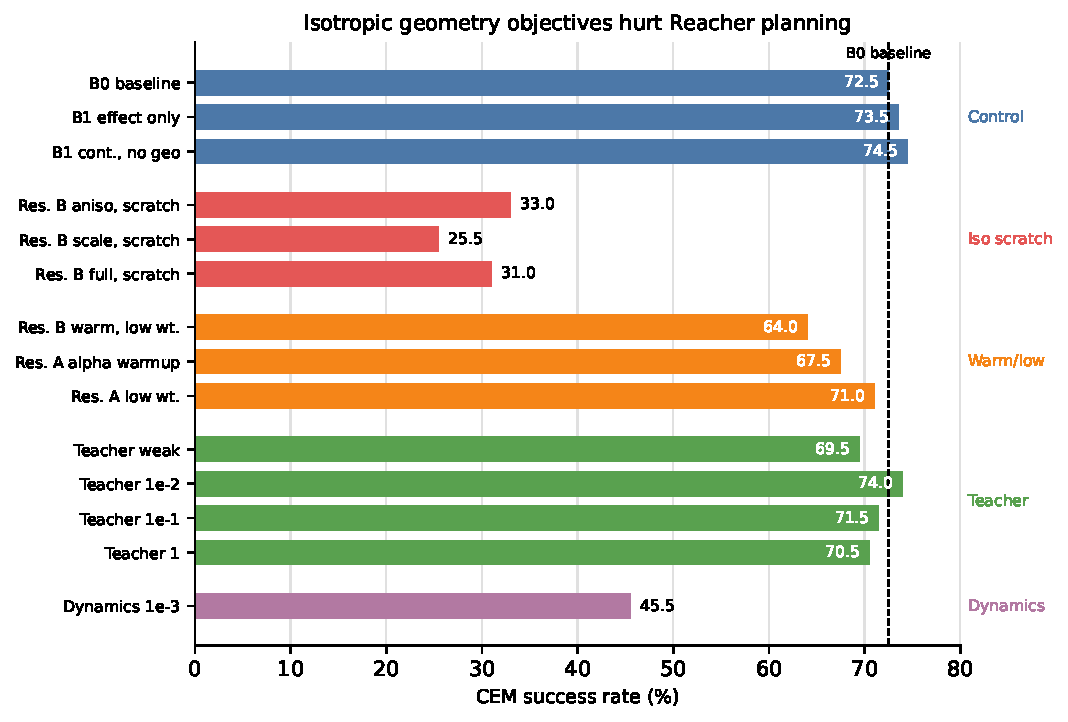
\includegraphics[width=\linewidth]{figures/isotropic_ablation_success.pdf}
    \caption{Reacher CEM success for geometry ablations.  The dashed line marks
    the B0 baseline.  From-scratch isotropic decompositions collapse far below
    baseline, while warm-started, lower-weight, and teacher-metric variants
    mostly recover toward baseline rather than producing a reliable gain.  This
    negative result motivates matching the environment metric instead of
    enforcing an isotropic reference metric.}
    \label{fig:isotropic-ablation}
\end{figure}

\subsection{Hypothesis 2: Preserve Environment Anisometry}
\label{sec:diagnostic-derivation}

The second hypothesis asks whether the true environment is locally
anisometric, and whether the learned model preserves that geometry.  Here
``anisometric'' simply means non-isometric in action space:
\(G_t\not\propto I\), so different action directions produce different local
effect magnitudes.  Let
\(E_\theta\) denote the frozen LeWM encoder.  For a fixed simulator state
\(x_t\) and action block \(\mathbf{a}_t\), define the true latent transition

\[
F^{\mathrm{env}}_t(\mathbf{a})
=
E_\theta\!\left(T_{\mathrm{env}}(x_t,\mathbf{a})\right),
\]

where \(T_{\mathrm{env}}\) is the simulator transition over the same effective
horizon used by LeWM.  The learned transition is

\[
F^{\mathrm{model}}_t(\mathbf{a})
=
P_\phi(\mathbf{z}_t,\mathbf{a}),
\qquad
\mathbf{z}_t = E_\theta(o_t).
\]

Both maps take the same normalized action coordinates into the same frozen
latent representation.  Their local Jacobians are

\[
J^{\mathrm{env}}_t
=
\left.
\frac{\partial F^{\mathrm{env}}_t(\mathbf{a})}
{\partial \mathbf{a}}
\right|_{\mathbf{a}=\mathbf{a}_t},
\qquad
J^{\mathrm{model}}_t
=
\left.
\frac{\partial F^{\mathrm{model}}_t(\mathbf{a})}
{\partial \mathbf{a}}
\right|_{\mathbf{a}=\mathbf{a}_t}.
\]

We estimate \(J^{\mathrm{env}}_t\) by simulator counterfactuals from the same
restored physical state,

\[
J^{\mathrm{env}}_t e_i
\approx
\frac{
E_\theta(o_{t+1}(\mathbf{a}_t+\epsilon e_i))
-
E_\theta(o_{t+1}(\mathbf{a}_t-\epsilon e_i))
}{2\epsilon},
\]

and compute \(J^{\mathrm{model}}_t\) by autograd with all network parameters
frozen.  These Jacobians induce pullback metrics on action space,

\[
G^{\mathrm{env}}_t
=
\left(J^{\mathrm{env}}_t\right)^\top J^{\mathrm{env}}_t,
\qquad
G^{\mathrm{model}}_t
=
\left(J^{\mathrm{model}}_t\right)^\top J^{\mathrm{model}}_t.
\]

For any small perturbation \(\Delta \mathbf{a}\),

\[
\|J_t\Delta \mathbf{a}\|_2^2
=
\Delta \mathbf{a}^{\top}G_t\Delta \mathbf{a}.
\]

Thus \(G_t\) is the local action-effect geometry.  A spherical \(G_t\) means
local isometry; an eccentric \(G_t\) means some action directions produce much
larger effects than others.

\paragraph{Metrics used in the tables.}
\begin{itemize}
  \item \(\boldsymbol{G_t=J_t^\top J_t}\): the local action metric.  Its
  quadratic form gives the squared latent-effect size caused by a small action
  perturbation.
  \item \(\boldsymbol{\kappa(G_t)}\): the condition number
  \(\lambda_{\max}(G_t)/\lambda_{\min}^{\mathrm{eff}}(G_t)\).  A value near
  \(1\) means locally isotropic; a large value means locally anisometric.  In
  two action dimensions, \(\sqrt{\kappa}\) is the ellipse axis ratio.
  \item \(\boldsymbol{\widetilde G_t}\): the trace-normalized metric,
  \[
  \widetilde G_t =
  G_t/(\operatorname{tr}(G_t)+\varepsilon).
  \]
  This removes absolute sensitivity scale and keeps only the shape and
  direction of the local metric.
  \item \(\boldsymbol{D_G(t)}\): the normalized metric-shape error,
  \[
  D_G(t)=
  \left\|
  \widetilde G^{\mathrm{model}}_t
  -
  \widetilde G^{\mathrm{env}}_t
  \right\|_F .
  \]
  Small \(D_G\) means the model and environment agree on the local geometry of
  actions; large \(D_G\) means the model has learned a different action
  geometry.
  \item \(\boldsymbol{D_\kappa(t)}\): the signed log-eccentricity distortion,
  \[
  D_\kappa(t)=
  \log \kappa(G^{\mathrm{model}}_t)
  -
  \log \kappa(G^{\mathrm{env}}_t).
  \]
  Positive values mean the model exaggerates anisometry; negative values mean
  it underestimates anisometry.
  \item \(\boldsymbol{E_\kappa(t)=|D_\kappa(t)|}\): the unsigned eccentricity
  error.  This measures mismatch size even when overestimates and
  underestimates would cancel in the signed mean.
  \item \(\boldsymbol{\Pr[\kappa_m>\kappa_e]}\): the fraction of evaluated
  states where the model is more eccentric than the environment.  This tests
  for a systematic bias rather than only an average error.
  \item \(\boldsymbol{\theta_1}\): the angle between the dominant eigenvectors
  of \(G^{\mathrm{env}}_t\) and \(G^{\mathrm{model}}_t\),
  \[
  \theta_{t,1}
  =
  \cos^{-1}
  \left(
  \left|
  \left(v^{\mathrm{env}}_{t,1}\right)^\top
  v^{\mathrm{model}}_{t,1}
  \right|
  \right)
  \cdot
  \frac{180}{\pi}.
  \]
  Small \(\theta_1\) means the model and environment agree on the dominant
  action-effect direction.  Large \(\theta_1\) means the planner is being told
  that a different raw action direction is most sensitive.
  \item \(\boldsymbol{\theta_{1:k}}\): the principal angles between the top
  \(k\)-dimensional eigenspaces.  If
  \(V^{\mathrm{env}}_{t,k}\) and \(V^{\mathrm{model}}_{t,k}\) contain the top
  \(k\) eigenvectors, then the singular values of
  \[
  \left(V^{\mathrm{env}}_{t,k}\right)^\top V^{\mathrm{model}}_{t,k}
  \]
  are the cosines of the principal angles.  These are important for Cube,
  where a single top eigenvector can be unstable but the dominant subspace may
  still be meaningful.
  \item \(\boldsymbol{\mathrm{effective\ rank}}\): the number of action
  directions that carry substantial metric mass.  Low effective rank means the
  local effect is concentrated in only a few action directions.
\end{itemize}

A useful conceptual object is the relative metric operator

\[
R_t
=
\left(G^{\mathrm{env}}_t+\delta_t I\right)^{-1/2}
G^{\mathrm{model}}_t
\left(G^{\mathrm{env}}_t+\delta_t I\right)^{-1/2}.
\]

In coordinates where the environment metric is locally whitened, the
eigenvalues of \(R_t\) quantify directional expansion or contraction of
predicted effects relative to true effects.  This operator states the ideal
comparison \(G^{\mathrm{model}}_t\sim G^{\mathrm{env}}_t\): if the two
geometries match, then \(R_t\) is close to a scaled identity.

\paragraph{How to read the experimental objects.}
\begin{itemize}
  \item Table~\ref{tab:isotropic-ablation} and
  Figure~\ref{fig:isotropic-ablation} test the old local-isometry hypothesis.
  They show that making the geometry spherical is not a reliable route to
  better planning.
  \item Table~\ref{tab:env-model} tests the new anisometry hypothesis.  It
  asks whether the environment is anisometric and whether pretrained LeWM
  learns the same anisometric metric.
  \item Figure~\ref{fig:local-metric-ellipses} visualizes the qualitative
  difference between the two environments.  Reacher is a direction-preserving
  eccentricity error; Cube is an eigenspace-rotation error.
  \item Figure~\ref{fig:cross-env-summary} gives the shared apple-to-apple
  diagnostics across Reacher and Cube.
  \item Table~\ref{tab:cube-epsilon} and Figure~\ref{fig:cube-robustness}
  check whether the Cube result is only a finite-difference/contact artifact.
\end{itemize}

\begin{figure}[t]
    \centering
    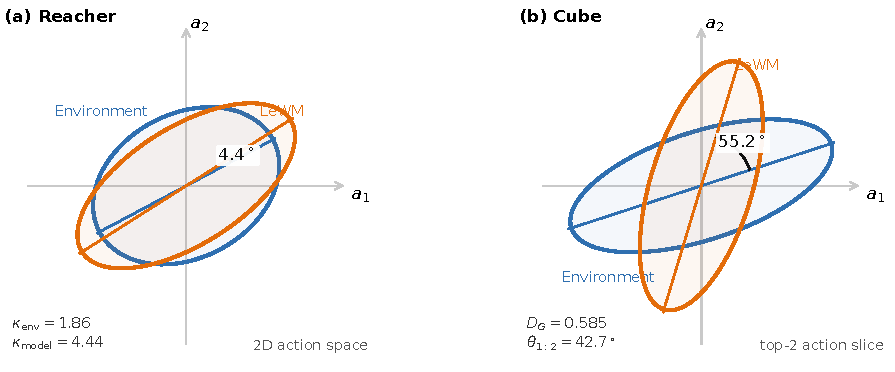
\includegraphics[width=\linewidth]{figures/local_metric_ellipses_reacher_cube.pdf}
    \caption{Schematic local action metrics induced by the environment and by
    pretrained LeWM.  Reacher is two-dimensional, so the ellipses directly
    visualize the action metric: LeWM preserves the dominant direction but
    exaggerates eccentricity.  Cube is five-dimensional, so the right panel is
    a top-two eigenspace cross-section; the main mismatch is eigenspace
    rotation rather than the Reacher-style direction-preserving eccentricity
    amplification.}
    \label{fig:local-metric-ellipses}
\end{figure}

\subsection{Anisotropic Environment--Model Test}
\label{sec:anisotropic-env-model-test}

The anisotropic test asks whether the model preserves the real local metric,
not whether either metric is close to the identity.  Table~\ref{tab:env-model}
summarizes the apple-to-apple comparison: pretrained LeWM, \(N=500\) states,
frameskip \(5\), normalized action coordinates, and
\(\epsilon=10^{-3}\).

The first answer is that both environments are anisometric.  Reacher is only
mildly anisometric, with median
\(\kappa(G^{\mathrm{env}})=1.86\).  Cube is strongly anisometric, with median
\(\kappa(G^{\mathrm{env}})\approx 3.0\times 10^3\).  Therefore the
environment itself does not support a universal local-isometry target.

The second answer is more important: pretrained LeWM does not simply recover
the environment metric.  In Reacher, it preserves the dominant direction very
well, with median top-1 angle \(4.41^\circ\), but exaggerates eccentricity:
median \(\kappa(G^{\mathrm{model}})=4.44\), median
\(D_\kappa=0.854\), and \(88.6\%\) of states have
\(\kappa_{\mathrm{model}}>\kappa_{\mathrm{env}}\).  In Cube, the mismatch is
not only eccentricity.  The dominant direction rotates by \(55.22^\circ\), and
the top-two eigenspace has a median maximum principal angle of
\(42.71^\circ\).  This suggests that the learned predictor can focus on
control-relevant prediction while inducing an action geometry that is
substantially different from the simulator's true local geometry.

\begin{table}[t]
\centering
\begin{tabular}{lccccccc}
\hline
Environment
& \(d_a\)
& \(D_G\)
& \(\kappa_{\mathrm{env}}\)
& \(\kappa_{\mathrm{model}}\)
& \(D_\kappa\)
& \(\Pr[\kappa_m>\kappa_e]\)
& top-1 angle \\
\hline
Reacher & 2 & 0.256 & 1.86 & 4.44 & 0.854 & 88.6\% & \(4.41^\circ\) \\
Cube    & 5 & 0.585 & \(3.0{\times}10^3\) & \(1.06{\times}10^4\) & 0.563 & 54.2\% & \(55.22^\circ\) \\
\hline
\end{tabular}
\caption{Environment--model local action geometry comparison.  \(D_G\) is the
Frobenius distance between trace-normalized metrics, and
\(D_\kappa=\log(\kappa_{\mathrm{model}}/\kappa_{\mathrm{env}})\).}
\label{tab:env-model}
\end{table}

\begin{figure}[t]
    \centering
    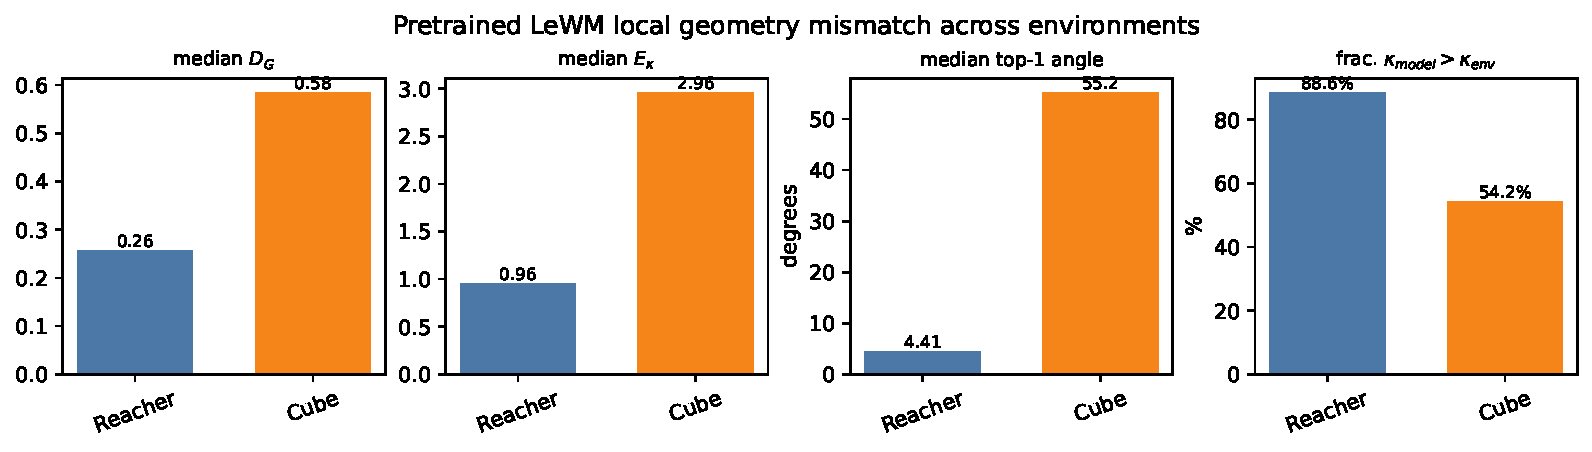
\includegraphics[width=\linewidth]{figures/cross_environment_geometry_summary.pdf}
    \caption{Shared geometry diagnostics for Reacher and Cube.  Reacher shows
    strong eccentricity amplification with good direction preservation.  Cube
    shows larger metric-shape error and much weaker dominant-direction
    alignment.}
    \label{fig:cross-env-summary}
\end{figure}

The two environments therefore support the same broad claim through different
mechanisms.  Reacher shows a precise direction-preserving eccentricity error:
the model knows which action direction matters most, but makes the local
metric too elongated.  Cube shows that the phenomenon is not confined to
two-dimensional action spaces: a pretrained prediction model can also learn a
different dominant action eigenspace.  This is the central empirical
observation for the workshop paper.

\subsection{Experiments and Robustness}
\label{sec:experiments-robustness}

For Reacher, the dominant direction is extremely well preserved: the median
top eigenvector error is \(4.41^\circ\).  However, the model condition number
is much larger than the environment condition number, and the median signed
distortion is \(D_\kappa=0.854\).  The corresponding absolute eccentricity
error is \(E_\kappa=0.956\).  Thus Reacher supports the hypothesis that LeWM
learns the main action-effect direction but exaggerates how different the
local action directions are.

For Cube, the main concern is finite-difference sensitivity around contacts.
We therefore repeat the environment Jacobian at
\(\epsilon\in\{10^{-3},3{\times}10^{-3},10^{-2}\}\).  The raw condition
numbers vary, as expected in a contact-rich manipulation domain, but the
shape and alignment conclusions are stable:

\begin{table}[t]
\centering
\begin{tabular}{ccccc}
\hline
\(\epsilon\)
& median \(D_G\)
& top-1 angle
& top-2 max angle
& effective rank env/model \\
\hline
\(10^{-3}\) & 0.585 & \(55.22^\circ\) & \(42.71^\circ\) & 1.959 / 2.355 \\
\(3{\times}10^{-3}\) & 0.541 & \(48.59^\circ\) & \(39.60^\circ\) & 2.002 / 2.355 \\
\(10^{-2}\) & 0.490 & \(45.87^\circ\) & \(35.95^\circ\) & 2.022 / 2.355 \\
\hline
\end{tabular}
\caption{Cube epsilon robustness.  The exact condition numbers are
epsilon-sensitive, but the metric-shape discrepancy and eigenspace mismatch
remain large across perturbation radii.}
\label{tab:cube-epsilon}
\end{table}

We also split Cube states by contact status using the dataset field
\(\texttt{proprio\_gripper\_contact}\).  A state is counted as contact if the
contact signal exceeds \(0.5\) at any point during the same five-step
transition used by LeWM.  This produces \(257\) non-contact and \(243\)
contact states.  The mismatch remains substantial even outside contact:
non-contact median \(D_G\) is \(0.508, 0.482, 0.427\) across the three
epsilons, and non-contact top-1 angle remains
\(47.84^\circ,43.91^\circ,36.06^\circ\).  Contact transitions make the
mismatch stronger, but they are not required for it.

\begin{figure}[t]
    \centering
    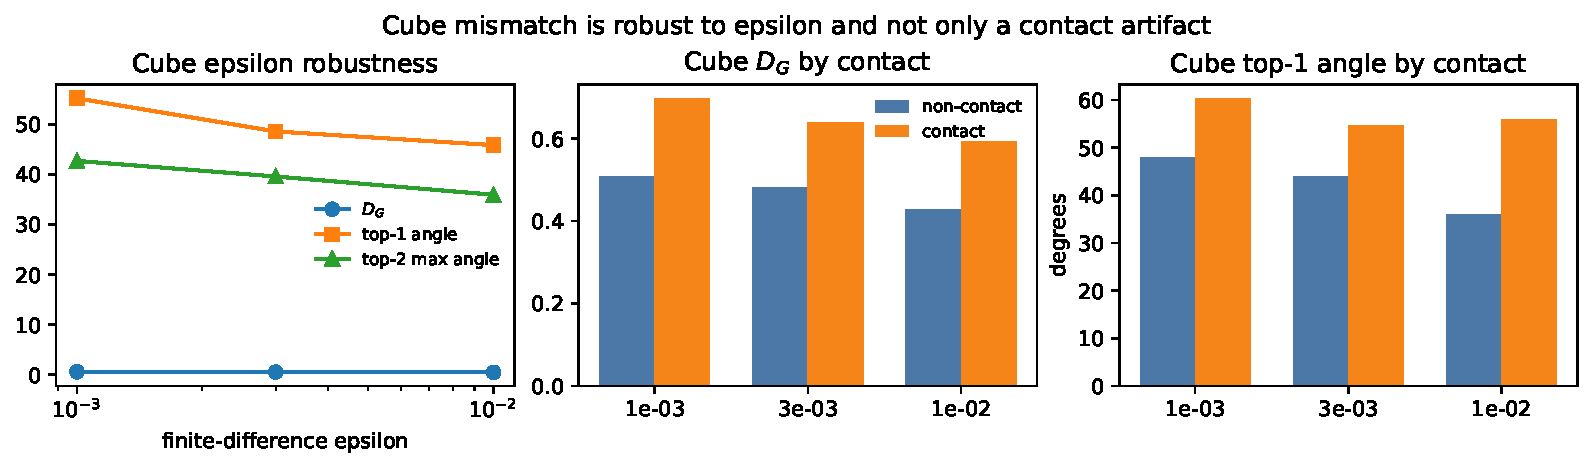
\includegraphics[width=\linewidth]{figures/cube_epsilon_contact_robustness.pdf}
    \caption{Cube robustness checks.  Left: aggregate mismatch remains large
    across finite-difference scales.  Middle and right: contact transitions
    increase the mismatch, but non-contact states still show large
    trace-normalized metric error and large top-eigenvector error.}
    \label{fig:cube-robustness}
\end{figure}

\subsection{Workshop Contribution and Next Direction}
\label{sec:workshop-contribution}

The resulting story is intentionally narrower than a full new algorithm.  The
paper's first contribution is to identify the geometric failure mode:
\begin{itemize}
  \item The old local-isometry hypothesis fails empirically.  Isotropic or
  self-referential geometry objectives can damage planning and do not provide
  a reliable improvement over LeWM.
  \item The environments themselves are anisometric.  Therefore the correct
  reference is not \(I\), but the environment-induced action metric
  \(G^{\mathrm{env}}_t\).
  \item Pretrained LeWM does not preserve this metric.  In Reacher it largely
  preserves orientation but exaggerates eccentricity; in Cube it learns a
  substantially different dominant eigenspace.
  \item This means the geometric problem is upstream of the proposed
  state-action scheme.  The next GeoJEPA objective should focus on preserving
  the true local action geometry, and only then ask how a state-action
  representation or practical non-oracle estimator can enforce it.
\end{itemize}

In short, the paper should not claim that local isometry is the answer.  The
more defensible workshop claim is that LeWM/LeJEPA-style predictors can distort
the local geometry of actions, and that preserving the environment's
anisometric action-effect metric is the problem that GeoJEPA should solve.

\end{document}
